\documentclass[tikz,border=10pt]{standalone}
\begin{document}
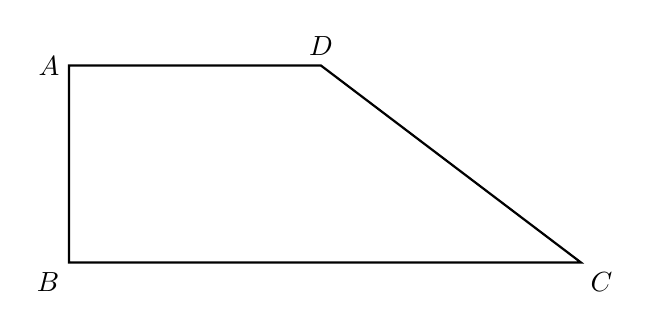
\begin{tikzpicture}
\coordinate (A) at (0,2.5);
\coordinate (B) at (0,0);
\coordinate (C) at (6.5,0);
\coordinate (D) at (3.2,2.5);

\draw[thick] (A) -- (B) -- (C) -- (D) -- cycle;

\node[anchor=east] at (A) {$A$};
\node[anchor=north east] at (B) {$B$};
\node[anchor=north west] at (C) {$C$};
\node[anchor=south] at (D) {$D$};
\end{tikzpicture}
\end{document}
